\section{Task taxonomy and measurement design}
\subsection{Typed contract and reference provenance}
An input comprises a state $s_i$ and a question map $Q_i$. Each question specifies an instruction, an output primitive and, when applicable, a candidate set or ordinal rubric. A \emph{choice} selects a finite label, a \emph{noul} returns a binary probability, and a \emph{score} returns a distribution over ordered levels together with its expectation. Model-facing payloads contain only state and questions; reference labels and hidden source metadata are excluded by an explicit whitelist.

The historical collection contains 15 source datasets or collections, instantiated as 28 main suites and eight repeat/reversal controls. Figure~\ref{fig:atlas} maps each source to an application domain and non-exclusive decision functions: semantic classification, routing, evidence use, ordinal judgment, safety, workflow, explicit rejection and retrieval. These functions are descriptive tags, not equal-weight components of a latent intelligence score. A suite additionally records primitive, language, candidate count, state/question multiplicity and reference type. Main-suite variants can share underlying examples: BoolQ and SST5, for example, each have two output encodings.

\begin{figure}[t]
\centering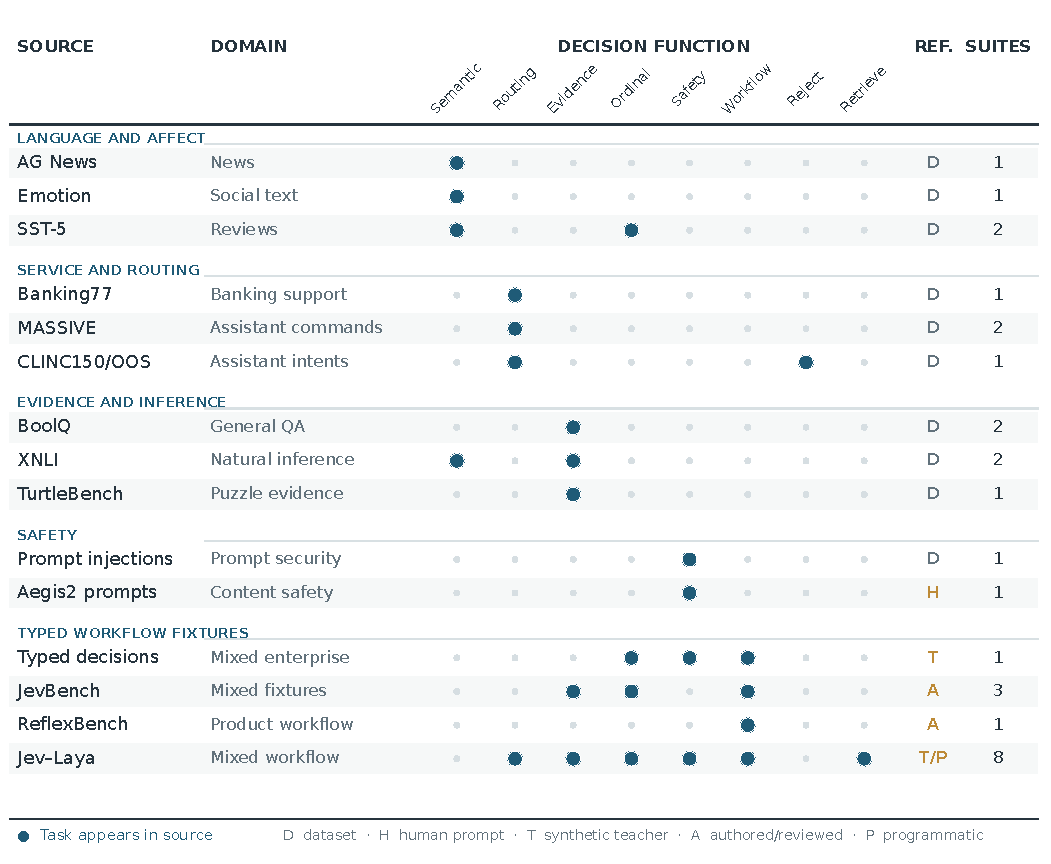
\includegraphics[width=.99\linewidth]{figures/fig_atlas.pdf}
\caption{Cross-domain source atlas. Rows are 15 source collections, grouped by application domain; filled cells mark non-exclusive decision functions. $S$ is the number of evaluated main suites, not independent datasets. Reference codes distinguish dataset labels (D), human prompt annotations (H), synthetic teachers (T), authored or AI-reviewed cases (A) and executable labels (P). The atlas classifies workload coverage, not model quality.}
\label{fig:atlas}
\end{figure}
\FloatBarrier

References are classified as dataset-provided, human prompt annotations, authored or AI-reviewed policy cases, synthetic-teacher outputs, or programmatic labels. Exact agreement with a synthetic teacher is reported as teacher agreement. The source manifest pins downloaded artifacts and preparation code; request fingerprints preserve dictionary insertion order because candidate order is an experimental variable. Original model outputs and input audits remain immutable.

\subsection{Correctness, discordance and paired effects}
Let $\hat y_i^{(a)}$ be the canonicalized finite prediction under condition $a$, and let $y_i$ be the reference. Invalid responses count as incorrect. Define $c_i^{(a)}=\mathbf{1}[\hat y_i^{(a)}=y_i]$. For a semantics-preserving intervention $a\!\to\!b$, we report
\begin{align}
\Delta_{a\to b}&=\frac{1}{n}\sum_i(c_i^{(b)}-c_i^{(a)}), &
D_{a\to b}&=\frac{1}{n}\sum_i\mathbf{1}[\hat y_i^{(a)}\ne\hat y_i^{(b)}].
\end{align}
These quantities answer different questions. If $N_{01}$ counts incorrect-to-correct changes and $N_{10}$ correct-to-incorrect changes, then $\Delta=(N_{01}-N_{10})/n$. The \emph{correctness turnover} $T=(N_{01}+N_{10})/n=|\Delta|+2\min(N_{01},N_{10})/n$ exposes the opposing changes hidden by net accuracy. Discordance $D$ also includes changed predictions that are both incorrect. We retain both transition counts, pair identifiers and source-cluster membership in the analysis artifact.

For candidate reversal, an original condition $o$, exact-repeat condition $r$ and reversed condition $v$ give the additional contrast $D_{r\to v}-D_{o\to r}$. This excess-discordance estimate uses the same clusters in both terms. It describes the implemented candidate presentation and answer-code mapping jointly. In the LLM adapter, changing candidate order also changes which answer code represents an option.

Uncertainty is estimated with 10,000 paired cluster-bootstrap draws and seed 20260929. The cluster is the source/state unit, including all questions and matched variants. Needle analyses resample the 25 original content units; their 450 derived states are not 450 independent samples. Intervals for historical contrasts are pointwise and descriptive. Complete contrast families, rather than only favorable directions, are retained.

\subsection{Compared systems}
The local systems are Laya English and Multilingual from the same pinned repository revision, Llama-3.1-8B-Instruct and Qwen3-8B. Laya uses native typed heads. The LLM adapter serializes each question and scores distinct single-token candidate codes with one forward pass, without generated reasoning. Its probabilities are conditional on those candidate logits. Supplied binary criteria and ordinal levels are preserved. All historical local decisions passed complete-input checks; checkpoint file hashes identify the actual local weights.

\paragraph{Hosted Jev.} The pinned \texttt{jev-1.13.0} endpoint completed 22,934 request executions covering the same 26,450 decisions. 8 decisions failed the declared transport/response validity rule and remain in the accuracy denominator. The API reported 23,841,873 input tokens, corresponding to USD 1.001 at the retrieved public price; unavailable usage on failed calls is not included. Every returned version and answer is retained. Server tokenization and weights are not observable. Hosted client times include the proxy, network and service and are reported separately from resident-GPU measurements.


\subsection{Fresh executable-policy diagnostic}
The new diagnostic generates 288 unique base states across refund, access-control and routing policies using three fixed data seeds. Original action labels are stratified, and boolean/ordinal marginal distributions are reported rather than assumed balanced. Each policy includes a priority-ordered action, an escalation predicate and a severity rule. The correct outputs are computed directly from visible facts and policy parameters and checked by a separately expressed rules implementation.

Eight matched variants test exact repetition, action-order reversal, an authored Chinese rendering, irrelevant archived records, question paraphrases, equivalent choice encodings, and a one-field counterfactual, alongside the original. The counterfactual must change the correct action; all other variants preserve the reference labels. Generation rejects base states without such a one-field intervention. Thus the diagnostic is a curated compositional-rule distribution. The generator, data fingerprints, scoring contract and intervention scope are frozen before inference. Three generator seeds replicate data generation, not model training.

All five systems complete 6,912 decisions each in this diagnostic. The six predeclared contrasts per model/policy family are excess reversal discordance, Chinese/distractor/paraphrase action correctness effects, and choice-encoding effects on review and severity correctness. We use a max-standardized-deviation bootstrap with 10,000 draws stratified by the three data seeds, providing simultaneous intervals within each six-effect family, not across models or policies. Zero empirical variance is flagged rather than interpreted as population invariance. A five-percentage-point practical discussion threshold was fixed before inference; it is not a universal acceptance criterion.

Each LLM additionally answers 1,440 codebook-control decisions: baseline, exact repeat, display-only reversal, code-only reversal and both. Prompt tests verify that baseline matches the ordinary adapter and both matches its reversed-candidate rendering. The native decision interfaces do not expose an equivalent answer-code assignment. These additional contrasts are descriptive and use pointwise intervals.

\subsection{Held-out wording challenge}
A post-hoc inspection of the fresh routing results motivated a second, separately frozen experiment. We generated 96 new base states from seeds 404, 505 and 606, disjoint from the 288-state policy set, balancing the four outage/payment truth cells within each seed. Each state has English and Chinese \emph{compact} and \emph{explicit} policy renderings. Within a language, only the first policy clause changes; facts, parameters, questions, answer options and executable references are held fixed. The preregistered primary contrast is explicit-minus-compact action accuracy on the 48 exclusive-or states in English; Chinese and the remaining truth cells are reported as secondary. All five systems completed 384 requests each. Intervals use 10,000 paired bootstrap draws stratified by seed and truth cell. This is a controlled wording test on authored policy text, not a human-validated translation study.
